\documentclass[a4paper,onecolumn,unpublished]{quantumarticle}
\pdfoutput=1
\usepackage{amsmath,amssymb,amsthm,mathtools}
\usepackage{graphicx}
\usepackage{booktabs}
\usepackage{tikz}
\usetikzlibrary{arrows.meta,positioning,calc}
\usepackage[numbers,sort&compress]{natbib}
\usepackage{hyperref}
\usepackage[capitalise,nameinlink]{cleveref}

\newtheorem{theorem}{Theorem}
\newtheorem{corollary}[theorem]{Corollary}
\newtheorem{proposition}[theorem]{Proposition}
\newtheorem{lemma}[theorem]{Lemma}
\theoremstyle{definition}
\newtheorem{definition}{Definition}
\theoremstyle{remark}
\newtheorem{remark}[theorem]{Remark}

\newcommand{\F}{\mathbb{F}_2}
\newcommand{\wt}{\operatorname{wt}}
\newcommand{\Wopt}{W_{\mathrm{opt}}}
\newcommand{\spn}{\operatorname{span}}
\newcommand{\qc}[1]{[\![#1]\!]}

\begin{document}

\title{No weight-four checks for $\qc{11,3,3}$: a certified computation of optimal check weights of small stabilizer codes}

\author{Yifan Jing$^{*}$}
\affiliation{University of Michigan, Ann Arbor, MI, USA}
\author{Yue Tu$^{*}$}
\affiliation{University of Michigan, Ann Arbor, MI, USA}

\maketitle
{\renewcommand{\thefootnote}{\fnsymbol{footnote}}\footnotetext[1]{These authors contributed equally.}}

\begin{abstract}
The check weight of a stabilizer code, the largest weight of a generator in a generating set of
its stabilizer group, governs the cost of syndrome extraction. Wei, Han, He, Li and Liu recently
determined the optimal check weight $\Wopt(n,k,d)$ of all qubit stabilizer codes with $n\le9$ and
left several entries with $10\le n\le12$ open. We prove that no $\qc{11,3,d\ge3}$ stabilizer code
admits a generating set of weight at most four, so that $\Wopt(11,3,3)=5$. This answers a question
recorded in the QIQCOP open-problem collection. We also give a $\qc{12,3,3}$ code with
weight-four generators, which shows that $12$ is the smallest length of an $\qc{n,3,3}$ code with
weight-four checks, and we determine six further entries:
$\Wopt(10,4,3)=6$, $\Wopt(11,4,3)=5$, $\Wopt(11,5,3)=7$, $\Wopt(12,4,3)=5$, $\Wopt(12,5,3)=6$ and
$\Wopt(12,6,3)=8$. The nonexistence proofs reduce the problem, through a syndrome formulation,
an induction on the length and a normal form under local Clifford operations and qubit
permutations, to finitely many Boolean satisfiability instances. Every instance is refuted with a
DRAT certificate checked by an independent checker. The complete argument for $\qc{11,3,3}$,
including every reduction and every satisfiability instance, is formalized in Lean~4, and all
new constructions are verified in Lean by kernel computation.
\end{abstract}

\section{Introduction}

Stabilizer codes~\cite{Got97,CRSS98} are specified by commuting Pauli operators, the checks,
whose eigenvalues are measured to detect errors. The weight of a check, the number of qubits on
which it acts, determines the size of the measurement circuit and how errors spread during syndrome
extraction. Low-weight checks are therefore a central requirement in fault-tolerant architectures
and in the theory of quantum low-density parity-check codes~\cite{BE21}, and constraints
such as two-dimensional geometric locality are known to limit what low-weight codes can
achieve~\cite{BPT10}.

Wei, Han, He, Li and Liu~\cite{WHHLL26} initiated a systematic theory of the \emph{optimal check
weight}. This is the quantity $\Wopt(n,k,d)$, defined as the least $w$ such that some $\qc{n,k,d}$ stabilizer code has a generating
set of weight at most $w$. They showed that computing the check weight of a given code is NP-hard,
proved analytical lower bounds, and combined a linear program for weight enumerators with explicit
constructions to determine $\Wopt(n,k,d)$ for all $n\le9$. For $10\le n\le12$ several entries of
their table remained open. One of them, whether $\Wopt(11,3,3)$ equals $4$ or $5$, is recorded as an open problem
in the QIQCOP collection~\cite{QIQCOP}. A weight-five $\qc{11,3,3}$ code is obtained from a
$\qc{9,3,3}$ code with weight-five generators by adding two qubits with single-qubit
checks~\cite{WHHLL26}, and neither the linear-programming bounds nor the known constructions decide
whether weight four is possible.

In this paper we settle this and several related entries.

\begin{theorem}
\label{thm:main}
No qubit stabilizer code with parameters $\qc{11,3,d}$, $d\ge3$, has a generating set whose
generators all have weight at most four. Hence $\Wopt(11,3,3)=5$.
\end{theorem}

\begin{theorem}
\label{thm:constructions}
There are stabilizer codes with parameters $\qc{12,3,3}$ and weight-four generators,
$\qc{10,4,3}$ with weight six, $\qc{11,4,3}$ with weight five, $\qc{11,5,3}$ with weight seven,
$\qc{12,4,3}$ with weight five, $\qc{12,5,3}$ with weight six and $\qc{12,6,3}$ with weight
eight. Moreover, no $\qc{11,5,3}$ code has generators of weight at most six.
\end{theorem}

Together with the lower bounds of Ref.~\cite{WHHLL26}, \cref{thm:main,thm:constructions}
determine all eight distance-three entries with $10\le n\le12$ that were open in
Ref.~\cite{WHHLL26} (\cref{tab:wopt}). Since $\Wopt$ is nonincreasing in $n$~\cite{WHHLL26},
\cref{thm:main} together with the $\qc{12,3,3}$ code shows that the least length of an
$\qc{n,3,3}$ code with weight-four checks is exactly $12$. Previously it was only known to lie
between $11$ and $15$~\cite{WHHLL26}, and the QIQCOP entry notes that a negative answer for
$n=11$ ``would leave the corresponding questions for $12\le n\le14$ open''~\cite{QIQCOP}.

\paragraph{Method and verification.}
Constructions are easy to check. Nonexistence is the hard direction, since the naive search
space consists of all eight-tuples of the $31\,714$ Pauli operators of weight at most four on
eleven qubits, about $10^{36}$ tuples. Our argument has three ingredients.
\begin{enumerate}
\item A \emph{syndrome formulation}. Every single-qubit error has a syndrome in $\F^{n-k}$, and the
distance condition becomes a statement about coincidences between these syndromes
(\cref{sec:syndromes}).
\item \emph{Reductions}. A code whose stabilizer contains a weight-one element reduces to a
shorter code. If it contains weight-two elements, a basis of their span can be taken as the first
generators and placed on fixed qubits. Local Clifford operations and qubit permutations bring the
remaining data to a normal form (\cref{sec:reductions}).
\item \emph{Certified satisfiability solving}. The remaining finitely many cases are encoded as
Boolean formulas and refuted by a SAT solver, which emits proof certificates that are checked
independently (\cref{sec:sat}).
\end{enumerate}
Computer-assisted proofs of this kind are established in combinatorics, for example for the
Boolean Pythagorean triples problem~\cite{HKM16} and Keller's conjecture~\cite{BHMN20}. The weak
points of such proofs are usually the hand-written reductions and encodings, not the solver. We
therefore also formalized the complete argument for \cref{thm:main} in the Lean~4 proof
assistant~\cite{Lean4,Mathlib}. The formal proof starts from the definition of a stabilizer code in
\cref{def:code}, proves every reduction, and discharges each satisfiability instance with Lean's
verified bit-blasting and certificate-checking tactic \texttt{bv\_decide}
(\cref{sec:lean}). As a sanity check, our encoders reproduce all thirteen distance-three values
of Ref.~\cite{WHHLL26} that we tested.

\section{Stabilizer codes and syndromes}
\label{sec:syndromes}

An $n$-qubit Pauli operator modulo phase is a vector $v=(a,b)\in\F^{2n}$, representing
$X^aZ^b=\bigotimes_jX^{a_j}Z^{b_j}$. Its weight is $\wt(v)=|\{j:(a_j,b_j)\ne(0,0)\}|$, and two
Pauli operators commute if and only if the symplectic form
$\langle(a,b),(a',b')\rangle=a\cdot b'+b\cdot a'$ vanishes. Following Ref.~\cite{QIQCOP} we use the
following definition, which includes degenerate codes.

\begin{definition}[Codes with bounded check weight]
\label{def:code}
Let $m=n-k$. Vectors $g_1,\dots,g_m\in\F^{2n}$ define an $\qc{n,k,d\ge3}$ stabilizer code with
check weight at most $w$ if (i) they are linearly independent; (ii) $\wt(g_i)\le w$ for all $i$;
(iii) $\langle g_i,g_{i'}\rangle=0$ for all $i,i'$; and (iv) every $v$ with $1\le\wt(v)\le2$ and
$\langle v,g_i\rangle=0$ for all $i$ lies in the span $S=\spn\{g_1,\dots,g_m\}$.
\end{definition}

Condition (iv) says that every Pauli operator of weight at most two that commutes with the
stabilizer is itself a stabilizer element up to phase, which is the condition $d\ge3$~\cite{KL97}.

\begin{remark}[Relation to the definition of Ref.~\cite{WHHLL26}]
\label{rem:def}
Ref.~\cite{WHHLL26} defines $\Wopt(n,k,d)$ over codes of distance exactly $d$ and minimizes over
arbitrary, possibly redundant, generating sets. The two definitions agree on every entry we
report. An independent subset of a generating set has the same span and no larger weight, so
independence is no restriction. A nonexistence statement for $d\ge3$ implies the one for $d=3$.
All our constructions have distance exactly three: besides $d\ge3$, we verified by exhaustive
search that each has a nontrivial logical operator of weight three.
\end{remark}

For a qubit $j$ and a Pauli type $t\in\{X,Y,Z\}$, let $e_{j,t}$ be the single-qubit error of type
$t$ on qubit $j$. Its \emph{syndrome} is $s_{j,t}=(\langle e_{j,t},g_i\rangle)_{i=1}^m\in\F^m$.
Writing $x_{ij}$ and $z_{ij}$ for the $X$- and $Z$-bits of $g_i$ on qubit $j$, we have
$s_{j,Z}=(x_{ij})_i$, $s_{j,X}=(z_{ij})_i$ and $s_{j,Y}=s_{j,X}+s_{j,Z}$. Two errors $e_{j,t}$ and
$e_{l,s}$ have equal syndromes exactly when their product commutes with every generator.

\begin{lemma}[Syndrome form of the distance condition]
\label{lem:syndrome}
Suppose (i)--(iii) of \cref{def:code} hold and $S$ contains no element of weight one. Then (iv)
holds if and only if (a) every syndrome $s_{j,t}$ is nonzero, which implies that (b) the three
syndromes on each qubit are pairwise distinct, and (c) whenever $s_{j,t}=s_{l,s}$ with $j\ne l$, the weight-two operator
$e_{j,t}+e_{l,s}$ lies in $S$. If $S$ contains no element of weight at most two, (iv) is equivalent
to all $3n$ syndromes being nonzero and pairwise distinct.
\end{lemma}

\begin{proof}
Operators of weight one are the $e_{j,t}$, and $e_{j,t}$ commutes with $S$ iff $s_{j,t}=0$.
Since $S$ has no weight-one elements, (iv) for weight one is exactly (a). Because
$s_{j,Y}=s_{j,X}+s_{j,Z}$, condition (a) is equivalent to (a) together with (b). Operators of
weight two are the $e_{j,t}+e_{l,s}$ with $j\ne l$, and such an operator commutes with $S$ iff
$s_{j,t}=s_{l,s}$; so (iv) for weight two is (c). In the pure case (c) forbids all coincidences
between different qubits.
\end{proof}

In the pure case the three syndromes on qubit $j$ are the nonzero vectors of a two-dimensional
subspace $V_j\subseteq\F^m$, and the distance condition says that $V_1,\dots,V_n$ intersect
pairwise trivially. This reformulation removes all auxiliary span-membership variables from the
pure case and makes the satisfiability instances much smaller.

\section{Reductions and normal forms}
\label{sec:reductions}

\begin{lemma}[Weight-one reduction]
\label{lem:reduce}
If generators satisfying \cref{def:code} for $(n+1,k,w)$ exist and $S$ contains an element of
weight one, then generators satisfying \cref{def:code} for $(n,k,w)$ exist.
\end{lemma}

\begin{proof}
Let $e\in S$ be supported on qubit $j_0$. Every element of $S$ commutes with $e$, so its component
on $j_0$ is $0$ or $e_{j_0}$. Deleting qubit $j_0$ from all elements of $S$ gives a subspace $S'$ of
dimension $m-1$, because the kernel of the deletion map on $S$ is spanned by $e$. Choose a basis of
$S'$ among the deletions of the $g_i$; weights do not increase. Commutation is inherited because
the $j_0$-components pairwise commute. If $v'$ on $n$ qubits has weight one or two and commutes
with $S'$, its extension by the identity on $j_0$ commutes with $S$, hence lies in $S$, and
deleting $j_0$ shows $v'\in S'$. Finally $k=(n+1)-m=n-(m-1)$.
\end{proof}

\begin{lemma}[Basis exchange]
\label{lem:exchange}
Let $g_1,\dots,g_m$ satisfy \cref{def:code} and let $b_1,\dots,b_r\in S$ be linearly independent
with $\wt(b_i)\le w$. Then there are generators $g'_1,\dots,g'_m$ satisfying \cref{def:code} with
the same span $S$, such that $g'_i=b_i$ for $i\le r$ and every $g'_i$ with $i>r$ is one of the
$g_j$.
\end{lemma}

\begin{proof}
Extend $\{b_i\}$ to a basis of $S$ using elements of $\{g_j\}$ (Steinitz exchange). Weights are at
most $w$, the span is unchanged, and so are (iii) and (iv).
\end{proof}

A local Clifford operation on qubit $j$ acts on the pairs $(x_{ij},z_{ij})$ by an invertible
$2\times2$ matrix over $\F$ and preserves weights and the symplectic form. On the syndromes of
qubit $j$ it permutes $\{s_{j,X},s_{j,Y},s_{j,Z}\}$, and since $GL(2,\F)\cong S_3$ every permutation
occurs. Qubit permutations permute the qubit index. Both operations preserve \cref{def:code} and
map $S$ to the corresponding transformed span.

\begin{lemma}[Normal form]
\label{lem:normal}
Order $\F^m$ lexicographically. If the three syndromes on each qubit are pairwise distinct, then
after local Clifford operations $s_{j,Z}<s_{j,X}<s_{j,Y}$ for every $j$. For any $t_0$, a
permutation of the qubits $j\ge t_0$ then makes $s_{j,Z}\le s_{j+1,Z}$ for all $j\ge t_0$.
\end{lemma}

\begin{proof}
Over $\F$ every invertible $2\times2$ matrix has determinant one, so $GL(2,\F)=Sp(2,\F)$ and every
local linear map preserves the symplectic form. It acts on the three nonzero syndromes of a qubit
by an arbitrary permutation, and we choose the one that sorts them. Local maps preserve supports.
The second step permutes only qubits $j\ge t_0$ and moves each qubit together with its three
syndromes, so the first normalization and any support constraints on qubits $j<t_0$ are kept.
\end{proof}

We now combine these ingredients. Fix a code as in \cref{def:code} with $w=4$ and $n\le11$, and
consider three exhaustive cases.
\begin{enumerate}
\item[(A)] \emph{$S$ contains a weight-one element.} By \cref{lem:reduce} a code of length $n-1$
with the same $k$ exists; we proceed by induction on $n$. For $n=k$ there are no generators and
(iv) fails, which is the base case.
\item[(B)] \emph{$S$ contains weight-two but no weight-one elements.} Let $W$ be the span of the
weight-two elements of $S$ and $r=\dim W\ge1$. Choose a basis of $W$ consisting of weight-two
elements and move it to the front with \cref{lem:exchange}. By \cref{lem:syndrome}(c) every
syndrome coincidence between different qubits is then explained by a combination of the first $r$
generators. For $r=1$ we permute the qubits so that $g_1$ is supported on $\{1,2\}$. For $r=2$ the
supports of $g_1$ and $g_2$ are equal, share one qubit, or are disjoint, and we place them on
$\{1,2\},\{1,2\}$, on $\{1,2\},\{2,3\}$, or on $\{1,2\},\{3,4\}$. In these layouts every element of
$W$ is supported on the first $t\le4$ qubits, so no coincidence involves a qubit $j>t$, and
\cref{lem:normal} applies with strict inequalities beyond $t$: two qubits $j,l>t$ with
$s_{j,Z}=s_{l,Z}$ would give a weight-two element of $W$ supported outside the first $t$ qubits.
For $r\ge3$ we place $g_1$ on $\{1,2\}$, require $\wt(g_i)\le2$ for $i\le r$, express collisions
through coefficient variables for the first $r$ generators, and sort the qubits $j\ge3$
non-strictly. The instance with parameter $r$ does not force $\dim W=r$; it only relaxes the
constraints, which is sound.
\item[(C)] \emph{$S$ contains no element of weight at most two (pure codes).} By
\cref{lem:syndrome} all $3n$ syndromes are distinct and nonzero, and \cref{lem:normal} gives a
strictly sorted normal form.
\end{enumerate}
In each case the normalized code yields an assignment to a Boolean formula that encodes the
weight bound, commutation, the syndrome conditions of \cref{lem:syndrome}, the supports fixed
above, and the normal form. \Cref{fig:flow} summarizes the case analysis. In the Lean
formalization each length $n\le11$ gives one pure instance, four instances for the layouts with
$r\le2$, and one instance for each $3\le r\le m$. The DRAT pipeline of \cref{sec:sat} uses a
coarser split for $n\le9$.

\begin{figure}[t]
\centering
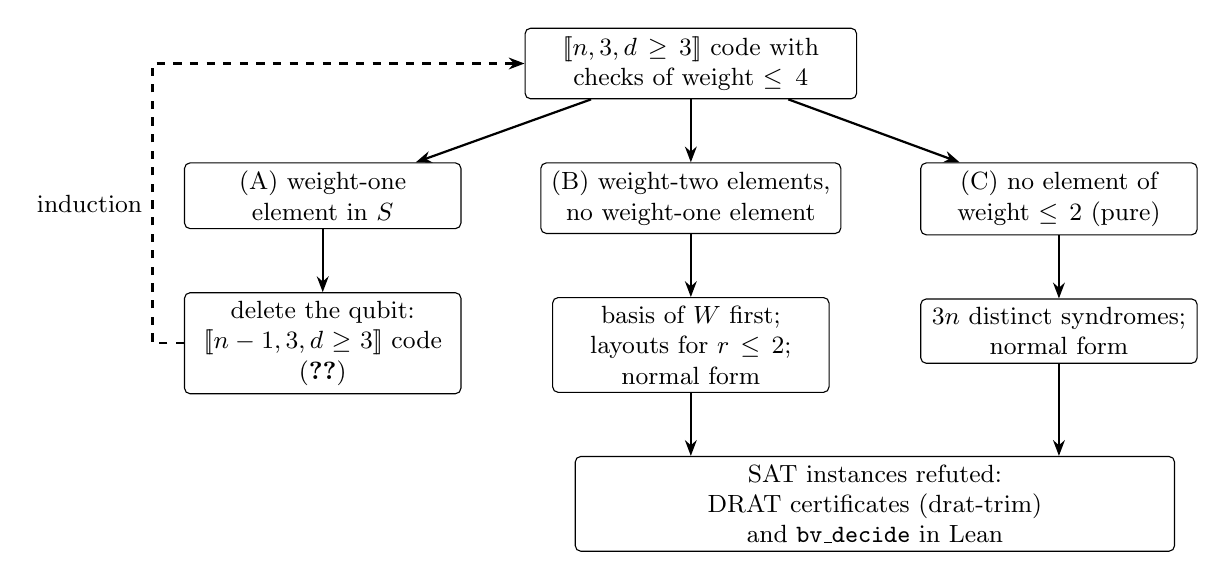
\begin{tikzpicture}[
  node distance=6mm and 5mm,
  box/.style={draw, rounded corners=2pt, align=center, font=\small, inner sep=3pt},
  every node/.append style={font=\small},
  arr/.style={-{Stealth[length=2mm]}, thick}]
\node[box, text width=40mm] (code) {$\qc{n,3,d\ge3}$ code with\\ checks of weight $\le4$};
\node[box, text width=33mm, below left=8mm and 8mm of code] (A) {(A) weight-one\\ element in $S$};
\node[box, text width=36mm, below=8mm of code] (B) {(B) weight-two elements,\\ no weight-one element};
\node[box, text width=33mm, below right=8mm and 8mm of code] (C) {(C) no element of\\ weight $\le2$ (pure)};
\node[box, text width=33mm, below=8mm of A] (A2) {delete the qubit:\\ $\qc{n-1,3,d\ge3}$ code\\ (\cref{lem:reduce})};
\node[box, text width=33mm, below=8mm of B] (B2) {basis of $W$ first;\\ layouts for $r\le2$;\\ normal form};
\node[box, text width=33mm, below=8mm of C] (C2) {$3n$ distinct syndromes;\\ normal form};
\node[box, text width=74mm, anchor=north] (sat) at ($(B2.south)!0.5!(C2.south |- B2.south)+(0,-8mm)$) {SAT instances refuted: DRAT certificates (drat-trim)\\ and \texttt{bv\_decide} in Lean};
\draw[arr] (code) -- (A);
\draw[arr] (code) -- (B);
\draw[arr] (code) -- (C);
\draw[arr] (A) -- (A2);
\draw[arr] (B) -- (B2);
\draw[arr] (C) -- (C2);
\draw[arr] (B2.south) -- (sat.north -| B2.south);
\draw[arr] (C2.south) -- (sat.north -| C2.south);
\draw[arr, dashed] (A2.west) -- ++(-4mm,0) |- node[pos=0.25, left, font=\small] {induction} (code.west);
\end{tikzpicture}
\caption{Structure of the proof of \cref{thm:main}. Every code falls into exactly one of three
cases. Case (A) reduces the length by one and is handled by induction, down to the trivial base
case $n=k$. Cases (B) and (C) are normalized and encoded as Boolean formulas, all of which are
unsatisfiable for $n\le11$.}
\label{fig:flow}
\end{figure}

\section{Satisfiability instances and certificates}
\label{sec:sat}

The variables of each instance are the bits $x_{ij},z_{ij}$ and, in case (B), coefficient bits
that express collisions as combinations of the first $r$ generators. Weight bounds are encoded
with sequential counters, parities with Tseitin variables, and lexicographic comparisons
bitwise. The Python CNF generators are part of the supplementary material.

For \cref{thm:main} we use, at each length $4\le n\le11$, one pure instance. For $n\le9$ case (B)
is encoded as a single instance in which $g_1$ is a weight-two element on qubits $\{1,2\}$ and
every collision must be explained by a combination of all $m$ generators, which is exactly
condition (iv); this only uses \cref{lem:exchange} with $r=1$. For $n=10,11$ this unified
encoding did not finish within an hour, and we split it into the four layouts with $r\le2$ and one
instance for each $3\le r\le m$. This gives $33$ instances. In the unified instances and the
instances with $r\ge3$ the qubits are not sorted, which only weakens these formulas. All
instances were solved with CaDiCaL~3.0.1~\cite{Cadical2}, which produced DRAT proofs, and all
proofs were checked with drat-trim~\cite{WHH14} (commit \texttt{2e3b2dc}). Every instance is
unsatisfiable and every certificate verified. On an Apple M1 Max laptop, $16$ of the $33$
instances take under a second. The hardest is the case $n=11$, $r=3$: solving takes about ten
minutes and checking about fourteen minutes. It is followed by the pure case at $n=11$, which
solves in about $1.5$ minutes. Exploratory runs used CaDiCaL through PySAT. The nonexistence part of \cref{thm:constructions}, for $\qc{11,5,3}$ with
weight six, uses the split encoding at lengths $6\le n\le11$, with base case $n=k=5$. For $m=1$
(length six) only the pure instance and the layout with $r=1$ occur. This gives
$2+5+6+7+8+9=37$ instances, all unsatisfiable with verified DRAT certificates.

\paragraph{Cross-validation.}
With the same pipeline we recomputed thirteen values of $\Wopt(n,k,3)$ that are known from
Ref.~\cite{WHHLL26}. All of them agree:
\begin{center}
\footnotesize\setlength{\tabcolsep}{3.2pt}
\begin{tabular}{l*{13}{c}}
\toprule
$(n,k)$ & $(5,1)$ & $(6,1)$ & $(7,1)$ & $(8,1)$ & $(8,2)$ & $(8,3)$ & $(9,1)$ & $(9,2)$ & $(9,3)$ & $(9,4)$ & $(10,1)$ & $(10,2)$ & $(10,3)$ \\
\midrule
$\Wopt$ & 4 & 4 & 4 & 4 & 4 & 6 & 4 & 4 & 5 & $\infty$ & 4 & 4 & 5 \\
\bottomrule
\end{tabular}
\end{center}
This tests both directions: the smallest feasible weight must be found, which exercises the
satisfiable case, and every smaller weight must be excluded. The value $\infty$ for $(9,4)$ means
that no code exists even without a weight bound. These runs used the split encoders through
PySAT and produced no certificates; they validate the encoders, not the proof.

\section{Formal verification in Lean}
\label{sec:lean}

We formalized \cref{thm:main} in Lean~4 with Mathlib~\cite{Lean4,Mathlib}. The final theorem
reads
\begin{center}
\texttt{theorem no\_weight\_four\_11\_3\_3 :}\\
\texttt{\ \ }$\neg\,\exists$\,\texttt{g :\ Fin 8} $\to$ \texttt{Pauli 11, IsCode 11 8 4 g}
\end{center}
where \texttt{IsCode n m w g} is \cref{def:code} verbatim: linear independence over
$\mathbb{Z}/2$, weights, commutation, and the span condition for all operators of weight one or
two. The development has about $1\,900$ hand-written lines for \cref{thm:main}, $1\,600$
generated lines for the satisfiability instances and $400$ lines for the constructions, and it
proceeds exactly as in \cref{sec:reductions}. It contains the invariance of \cref{def:code} under qubit permutations and
local linear maps, the basis exchange, the weight-one reduction, the local Clifford normal form
and sorting, the translation from a normalized code to Boolean data, and the case analysis
(A)--(C) with induction on $n$.

The Boolean specifications of cases (B) and (C) are Lean definitions with bounded quantifiers.
Each of the $61$ instances for $4\le n\le11$ is stated as a Lean theorem and proved by first
expanding the quantifiers and then calling \texttt{bv\_decide}. This tactic bit-blasts the formula
inside Lean, calls CaDiCaL, and checks the resulting LRAT certificate~\cite{CHHKS17} with a checker
verified in Lean. Lean thus verifies its own Boolean specification and the decomposition into
cases; the Python CNF files of \cref{sec:sat} are an independent second implementation. The
Lean instances omit the linear-independence constraint, which only strengthens them. The trusted
base consists of the Lean kernel, Mathlib's definitions, and the Lean compiler and runtime, which
evaluate the certificate checker; the last dependency appears as $49$ auxiliary axioms in the
output of \texttt{\#print axioms}, one for each instance that is not already closed by the
preprocessing (twelve small instances are). The step from $\Wopt$ to \cref{def:code} is
\cref{rem:def}. We used Lean \texttt{v4.35.0-rc2} and Mathlib at revision
\texttt{0653561}. Building the instances for $n=11$ requires up to about $20$\,GB of memory
and a few hours of CPU time.

All seven constructions of \cref{thm:constructions} are verified in Lean by kernel computation
(\texttt{decide}): commutation, weights, linear independence via an explicit dual basis, and the
absence of commuting operators of weight one or two, which gives $d\ge3$. These theorems depend
only on Lean's standard axioms. The nonexistence of weight-six $\qc{11,5,3}$ codes is certified by DRAT but not
formalized in Lean.

\section{Constructions and updated table}
\label{sec:results}

The $\qc{12,3,3}$ code is shown in \cref{fig:code12}. It is pure: all $36$ single-qubit syndromes
are nonzero and pairwise distinct, so its distance is at least $3$. It has a nontrivial logical
operator of weight three, so the distance is exactly $3$ (\cref{rem:def}). The other constructions of
\cref{thm:constructions} are listed in \cref{app:codes}; all of them are pure as well.
\Cref{tab:wopt} shows the distance-three entries of Table~II of Ref.~\cite{WHHLL26} for
$10\le n\le12$ together with the values established here.

\begin{figure}[t]
\centering
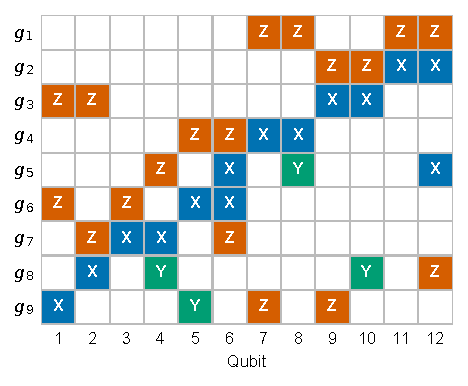
\includegraphics[width=0.62\linewidth]{figures/fig_code12.pdf}
\caption{Generators $g_1,\dots,g_9$ of a $\qc{12,3,3}$ stabilizer code with checks of weight
four. Colored cells show the Pauli operator of each generator on each qubit (blank: identity).
The generators commute pairwise and are linearly independent, and the $36$ single-qubit syndromes
are nonzero and pairwise distinct, so the code is pure with distance at least three; a weight-three
logical operator shows that the distance is exactly three.}
\label{fig:code12}
\end{figure}

\begin{table}[t]
\centering
\begin{tabular}{lcccccc}
\toprule
 & $k=1$ & $k=2$ & $k=3$ & $k=4$ & $k=5$ & $k=6$ \\
\midrule
$n=10$ & 4 & 4 & 5 & \textbf{6} (6--7) & $\infty$ & $\infty$ \\
$n=11$ & 4 & 4 & \textbf{5} (4--5) & \textbf{5} (5--7) & \textbf{7} (6--8) & $\infty$ \\
$n=12$ & 4 & 4 & \textbf{4} (4--5) & \textbf{5} (5--7) & \textbf{6} (6--8) & \textbf{8} (8--10) \\
\bottomrule
\end{tabular}
\caption{Optimal check weight $\Wopt(n,k,3)$ for $10\le n\le12$ and $k\le6$. Bold entries were open
in Ref.~\cite{WHHLL26}, and the previous bounds are given in parentheses. Lower bounds for the
bold entries come from Ref.~\cite{WHHLL26}, except for $\Wopt(11,3,3)\ge5$ (\cref{thm:main}) and
$\Wopt(11,5,3)\ge7$ (\cref{thm:constructions}). Upper bounds come from our constructions, except
for $\Wopt(11,3,3)\le5$~\cite{WHHLL26}. Remaining entries are as in Ref.~\cite{WHHLL26}.}
\label{tab:wopt}
\end{table}

\section{Discussion}
\label{sec:discussion}

\Cref{thm:main} answers the QIQCOP question~\cite{QIQCOP} negatively, and the $\qc{12,3,3}$
construction answers the follow-up question for lengths $12\le n\le14$. The method depends on
three features that are common to many finite questions about stabilizer codes: syndromes turn
distance conditions into injectivity constraints; low-weight stabilizer elements can be moved to
the front and placed on fixed qubits; and the symmetry group of local Clifford operations and qubit
permutations admits a simple normal form. We expect the same approach to apply to other small
entries of the check-weight table, including distance four, where the syndrome conditions involve
pairs of errors.

The two layers of certification play different roles. DRAT certificates make the solver
untrusted but still rely on the correctness of the encoding, which we also cross-validated against
thirteen known values. The Lean formalization removes the trust in the encoding and in the
reductions and leaves the Lean kernel, Mathlib's definitions and the Lean compiler. In our view,
this combination is a practical way to make computer-assisted results in quantum coding theory
checkable.

\section*{Acknowledgments}
The reduction strategy, the satisfiability encodings and the Lean formalization were developed with
the assistance of Claude (Anthropic). The authors checked all arguments and take full
responsibility for the content. We thank the maintainers of the QIQCOP collection for curating the
problem and F.~Wei, Z.~Han, A.~Y.~He, Z.~Li and Z.-W.~Liu for their table of optimal check
weights.

\section*{Code availability}
The Lean formalization, the SAT encodings, the certificate logs and the scripts are available at
\textbf{[repository URL to be added]}.

\appendix
\section{Generators of the new codes}
\label{app:codes}

Each string lists the Pauli operator of one generator on qubits $1,\dots,n$.

\begin{center}
\small
\begin{tabular}{llll}
\toprule
$\qc{10,4,3}$, $w=6$ & $\qc{11,4,3}$, $w=5$ & $\qc{11,5,3}$, $w=7$ & $\qc{12,4,3}$, $w=5$ \\
\midrule
\texttt{IZIZIZZZIZ} & \texttt{ZIZZIIIIIZZ} & \texttt{IIIZIZZZZZZ} & \texttt{IIIIIIIZZZZZ} \\
\texttt{IIIZZZIZZZ} & \texttt{IZIZIIZZZII} & \texttt{IZZIZIIXXXX} & \texttt{IIIZIIIIXXXX} \\
\texttt{ZIIIIXXXXX} & \texttt{ZIIIZZIZIZI} & \texttt{IIIXXXXIYXX} & \texttt{IIIIZZZXIIIX} \\
\texttt{ZIZXXIIIYY} & \texttt{IIIIIIZXXXX} & \texttt{IXXIIYXZIXY} & \texttt{IIIXXXXIIIIZ} \\
\texttt{ZXXZXIIXII} & \texttt{IIIXXXXIIIY} & \texttt{ZIXIYZYYIZI} & \texttt{IZZZIYXIIIII} \\
\texttt{XIYIXZYIIY} & \texttt{IXXIIXXIIYI} & \texttt{XYIIYYYIYIY} & \texttt{IXXIIIIIIZZI} \\
                    & \texttt{XIYIYIYIYII} &                     & \texttt{ZIZIXIIYIIXI} \\
                    &                      &                     & \texttt{XIYIIIYIIYIY} \\
\bottomrule
\end{tabular}

\vspace{1em}
\begin{tabular}{lll}
\toprule
$\qc{12,3,3}$, $w=4$ & $\qc{12,5,3}$, $w=6$ & $\qc{12,6,3}$, $w=8$ \\
\midrule
\texttt{IIIIIIZZIIZZ} & \texttt{IZIIZIIIZZZZ} & \texttt{IIIIZZZZZZZZ} \\
\texttt{IIIIIIIIZZXX} & \texttt{IIIIIIZZXXXX} & \texttt{ZIIZIIXXXXXX} \\
\texttt{ZZIIIIIIXXII} & \texttt{IIZZZZXXIIII} & \texttt{IIZZXXZIIIXY} \\
\texttt{IIIIZZXXIIII} & \texttt{IIXXXXIIIIZY} & \texttt{IZIXYXIYYXIY} \\
\texttt{IIIZIXIYIIIX} & \texttt{IXIYYXXYIIII} & \texttt{IXXIIXXIYXYX} \\
\texttt{ZIZIXXIIIIII} & \texttt{ZZIIIYIYIXYI} & \texttt{XIYYIIYYZYIX} \\
\texttt{IZXXIZIIIIII} & \texttt{XIZIXIYIZIXI} & \\
\texttt{IXIYIIIIIYIZ} & & \\
\texttt{XIIIYIZIZIII} & & \\
\bottomrule
\end{tabular}
\end{center}

\bibliographystyle{quantum}
\bibliography{references}

\end{document}
